\chapter{QUADRO TEÓRICO}

	\par Neste capítulo serão descritos os principais conceitos e características
das tecnologias utilizadas para o desenvolvimento desta pesquisa.
	
	%Java
	\section{Java}
		\section{\textit{Java}}

	\par Conforme \citeonline{deitel2010}, \textit{Java} é uma linguagem de
programação orientada objetos, baseada na linguagem C++, desenvolvida pela
empresa \textit{Sun Microsystem} no ano de 1995, por uma equipe sob liderança
de James Gosling.

	\par Segundo \citeonline{caelum3}, para executar as aplicações, o
\textit{Java} utiliza uma máquina virtual denominada JVM\footnote{JVM - Java
Virtual Machine}, que liberta os softwares de ficarem presos a um único sistema
operacional, uma vez que o programa conversa diretamente com a JMV e fica por
conta dela traduzir os \textit{bytecodes} gerados pelo compilador para
linguagem de máquina.

	\par De acordo com \citeonline{java}, o \textit{Java} está presente em mais de
um bilhão de dispositivos como celulares, computadores, consoles de
\textit{games} e pode ser considerado, seguro, rápido e confiável.

	\par Hoje, com a acenção do \textit{Android}, a tendência é aumentar cada vez
mais o desenvolvimento em \textit{Java}, uma vez que os aplicativos Android são
desenvolvidos nessa linguagem. Nessa pesquisa a linguagem de programação
\textit{Java} será utilizado no desenvolvimento tanto do aplicativo quanto do
\textit{web service}.

	%Android
	\section{Android}
		%\section{Android}

	\par Segundo \citeonline{monteiro2012}, Android é um sistema operacional
baseado em Linux, que utiliza a linguagem de programação Java para o
desenvolvimento de seus aplicativos. Criado especialmente para dispositivos
móveis, começou a ser desenvolvido no ano de 2003 pela então empresa Android
Inc, que em 2005 foi agregada ao Google. A partir de 2007 o projeto Android
uniu-se a Open Handset Alliance, uma associação de empresas de
softwares, hardwares e telecomunicações, que tem por finalidade desenvolver uma
plataforma para dispositivos móveis que seja completa, aberta e gratuita.

	\par \citeonline{krazit2009} afirma que o sistema pode rodar em equipamentos
de diversos fabricantes, evitando assim ficar limitado a poucos dispositivos.
Conforme informações do site \citeonline{android1}, hoje em dia existe mais de
um bilhão de aparelhos espalhados pelo mundo com esse sistema operacional.

	\par De acordo com \citeonline{monteiro2012}, as aplicações são executadas em
uma máquina virtual Java denominada Dalvik. Cada aplicativo, usa uma instância
dessa máquina virtual, tornando-o assim mais seguro. Por outro lado, os
softwares só podem acessar os recursos do dispositivo, como uma lista de
contatos, caso seja formalmente aceito pelo usuário nos termos de uso, ao
instalá-lo.

	\par As configurações de uma aplicação na plataforma Android ficam salvas em um
arquivo XML\footnote{XML - \textit{Extensible Markup Language}.} denominado
\texttt{AndroidManifest.xml}, que se localiza na pasta raiz do projeto. Para
\citeonline{lecheta2010}, as informações devem estar entre \textit{tags}
correspondentes ao recurso.

	\par \citeonline{lecheta2010} diz que as Intents são recursos tão importantes
que podem ser consideradas como o coração do Android e que estão presentes em
todas as aplicações.	De acordo com \citeonline[p.29]{k192012}, "Intents são
objetos responsáveis por passar informações, como se fossem mensagens, para os
principais componentes da API do Android, como as Activities, Services e
BroadCast Receivers". \citeonline{monteiro2012} diz que as Intents são criadas
quando se tem a intenção de realizar algo como por exemplo compartilhar uma
imagem, utilizando os app's já existentes no dispositivo. Existem dois tipos de
Intents:
	
	\begin{itemize}
	  
	  \item Intents implícitas: quando não é informada qual activity deve ser
	  chamada, ficando assim por conta do sistema operacional verificar qual é a
	  melhor opção.
	  
	  \item Intents explícitas: quando é informada qual activity deve ser chamada.
	  Usada normalmente para chamar \textit{activities} da mesma aplicação.
	  
	\end{itemize}
	
	\par Segundo \citeonline{k192012}, uma aplicação Android pode ser construída
com quatro tipos de componentes: Activity, Services, Content Providers e
Broadcast Receivers.

	\par As \textit{activities} são as telas com interface gráfica, que permitem
interações com os usuários. De acordo com \citeonline{lacheta2013}, cada
\textit{activity} tem um ciclo de vida, uma vez que ela pode estar sendo
executada, estar em segundo plano ou totalmente destruída.

	\par Toda vez que é iniciada uma activity, ela vai para o topo de uma pilha
denominada \textit{activity stack}. O bom entendimento de seu ciclo de vida é
importante, pois quando uma aplicação é interrompida, é possível salvar as
informações ou ao menos voltar ao estágio a qual o usuário se encontrava. Na
Figura \ref{fig:qt1} é demonstrado o ciclo de vida de uma \textit{activity}.

	\begin{figure}[h!]
		\centerline{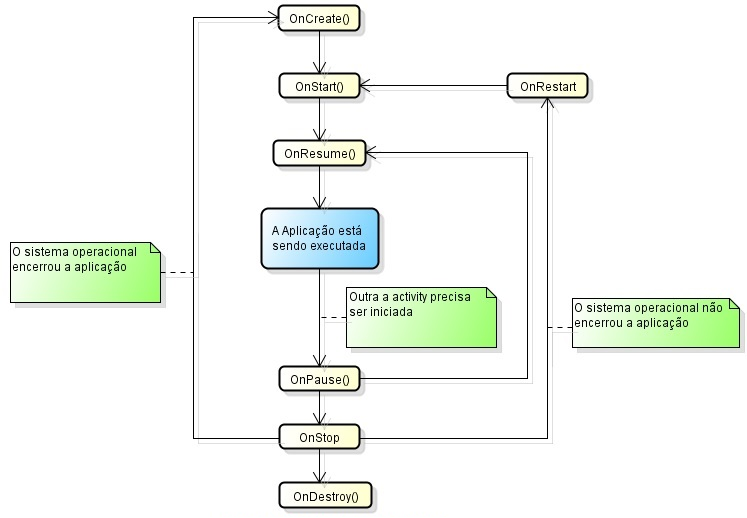
\includegraphics[scale=0.8]{./imagens/1_q_teorico/qt1.png}}
		\caption[Ciclo de Vida de uma Activity]{Ciclo de Vida de uma
		Activity.
		 \textbf{Fonte:}\citeonline{lecheta2010}}
		\label{fig:qt1}
	\end{figure}

	\par Para que se possa entender melhor, imagina-se o seguinte cenário: um
usuário entra no aplicativo de notas da Univás. Para que a \textit{activity}
seja criada, é chamado o método \texttt{onCreate()}, logo após é executado o
método \texttt{onStart()} e ao finalizar do ciclo anterior é chamado o
\texttt{onResume()}, só a partir de então, a \textit{activity} é visualizada
pelo discente. Contudo, durante a navegação, o aluno recebe uma ligação, então
nessa hora o sistema operacional chama o método \texttt{onPause()} para
interromper a aplicação e abrir uma outra \textit{activity} para que o usuário
possa atender a chamada telefônica. É possível, nesse método, salvar
informações que o usuário está utilizando. Ao concluir o método de pausa, é
executado o método \texttt{onStop()}, a partir de agora a \textit{activity} da
Univás não será mais visível ao usuário.

 	\par Ao encerrar a ligação, há dois caminhos possíveis de se percorrer, o
primeiro, seria o caso do sistema operacional encerrar completamente a
aplicação, por necessidade de liberar espaço em memória. Para destrui-la é
chamado o método \texttt{onDestroy()}. Dessa forma, para executar o aplicativo
da Univás será necessário chamar o método \texttt{onCreate()} novamente
seguindo o ciclo normal. Porém se não for encerrada completamente, ao findar a
ligação será executado o método \texttt{onRestart()} e voltar para a
\textit{activity} ao qual o usuário se encontrava.

	\par No arquivo \texttt{AndroidManifest.xml} as \textit{activities} devem estar
entre as tags \texttt{<activity> </activity>} e a \textit{activity} principal,
ou seja, pela qual será iniciada a aplicação deve conter a \textit{tag}
\texttt{<intent-filter>} além de \texttt{<action
android:name="android.intent.action.MAIN"/>} indicando que essa atividade
deverá ser chamada ao iniciar a aplicação e \texttt{<category
android:\\name="android.intent.category.LAUNCHER"/>} que implica que esse
APP ficará disponível junto aos outros aplicativos no dispositivo.
Na figura \ref{fig:qt2} é apresentado o código do arquivo
\texttt{AndroidManifest.xml}. Nela, pode-se ver o nome da classe que será
iniciada e no atributo \textit{label} o nome que aparecerá na tela para o
usuário.
	
	\begin{figure}[h!]
		\begin{lstlisting}[style=custom_XML]
		  <activity
	            android:name=".MainActivity"
	            android:label="@string/app_name" >
	            <intent-filter>
	                <action android:name="android.intent.action.MAIN" />
	                <category android:name="android.intent.category.LAUNCHER" />
	            </intent-filter>
	      </activity>
		\end{lstlisting}
		\caption[Código do arquivo
		AndroidManifest.xml indicando qual activity deve ser executada quando a
		aplicação iniciar]{Código do arquivo \texttt{AndroidManifest.xml} indicando
		qual \textit{activity} deve ser executada quando a aplicação iniciar.
		 \textbf{Fonte:}Elaborado pelos autores}
		\label{fig:qt2}
	\end{figure}
	
	\par A \textit{Activity} a ser utilizada para iniciar a aplicação é uma
\texttt{Navigation Drawer}, que segundo o site \citeonline{android2015}, ela exibe
do lado esquerdo as principais funções do software, semelhante a um
menu, que fica normalmente escondida aparecendo apenas quando clicado no canto
superior esquerdo. 

	\par Segundo \citeonline{lecheta2010}, a classe \texttt{Service} existe com o intuito
de executar processos que levarão um tempo indeterminado para serem executados
e que normalmente consomem um alto nível de memória e processamento. Esses
processos são executados em segundo plano enquanto o cliente realiza outra
tarefa. Assim um usuário pode navegar na internet enquanto é feito um
\textit{download}. O serviço é geralmente iniciado pelo \texttt{Broadcast Receiver} e
quem o gerencia é o sistema operacional que só o finalizará ao concluir a
tarefa, salvo quando o espaço em memória é insuficiente.

	\par Para \citeonline{lecheta2010}, um \texttt{Content Provider} provê conteúdos de
forma pública para todas as aplicações, possibilitando aos aplicativos consultar,
salvar, deletar e alterar informações no \textit{smartphone}. Assim afirma
\citeonline[p.413]{lecheta2010} “o Android tem uma série de provedores de
conteúdo nativos, como, por exemplo, consultar contatos da agenda, visualizar
os arquivos, imagens e vídeos disponíveis no celular”. Portanto, um contato
pode ser salvo na agenda de contatos do dispositivo por um aplicativo e
alterado por outro.

	\par Para \citeonline{monteiro2012}, o \texttt{Broadcast Receiver},
é um componente do Android responsável por responder a eventos do sistema.
Ele não possui interface gráfica e normalmente interage com os usuários através
de notificações.

	\par Outra ferramenta importante e muito utilizada do Android é a Notificação.
Segundo \citeonline{phillips2013} quando uma aplicação está sendo
executada em segundo plano e necessita comunicar-se com o usuário, o aplicativo
cria uma notificação. Normalmente as notificações aparecem na barra superior, o
qual pode ser acessado arrastando para baixo a partir da parte superior da
tela. Assim que o usuário clica na notificação ela cria uma \textit{activity}
para abrir  aplicação em questão.

	\par O Android traz embarcado em sua plataforma o banco de dados
\texttt{SQLite}, que armazena tabelas, \textit{views}, índices,
\textit{triggers} em apenas um arquivo em disco. Somente é possível acessa-lo
pela aplicação a qual o criou e, é deletado caso o aplicativo seja removido.

	\par Na seção abaixo serão descritos os elementos gráficos presentes no
Android.

	

		%elementos gráficos
		\subsection{Elementos Gráficos}
			%\subsection{Elementos Gráficos}
	
	\par Em uma aplicação, um elemento fundamental é a interface gráfica, que
deverá ser organizada, simples e elegante. O Android organiza os elementos
gráficos (\textit{widgets}) através de \textit{layouts} Conforme
\citeonline{monteiro2012} esses são os principais \textit{layouts} do sistema
operacional Android:
	
		\begin{itemize}
		
			\item LinearLayout: permite posicionar os elementos em forma linear, dessa
			forma quando o dispositivo estiver em forma vertical os itens ficarão um
			abaixo do outro e quando estiver na horizontal eles ficarão um ao lado do
			outro.
			
			\item RelativeLayout: permite posicionar elementos de forma relativa, ou
			seja um \textit{widget} com relação a outro.
			
			\item TableLayout: permite criar \textit{layouts} em formato de tabelas. O
			elemento TableRow representa uma linha da tabela e seus filhos são as
			células.  Dessa maneira, caso um TableRow possua dois itens, significa que
			essa linha tem duas colunas.
			
			\item DatePicker: \textit{widget} desenvolvido para a seleção de datas que
			podem ser usadas diretamente no \textit{layout} ou através de caixas de
			diálogo.
		
			\item Spinner: \textit{widget} que permite a seleção de itens, similar ao
			\textit{combobox}.
			
			\item ListViews: permite exibir itens em uma listagem. Dessa forma, em uma
			lista de compras, clicando em uma venda, é possível listar os detalhes dessa
			venda selecionada.
			
			\item Action Bar: um item muito importante, pois apresenta na parte superior
			aos usuários as opções existentes no aplicativo.
			
			\item AlertDialog: apresenta informações aos usuários através de uma caixa
			de diálogo. Comumente utilizado para perguntar ao cliente o que deseja fazer
			quando ele seleciona algum elemento.
			
			\item ProgressDialog e ProgressBar: utilizado quando uma aplicação necessita
			de um recurso que levará um certo tempo para executar, como por exemplo,
			fazer um \textit{download}, pode ser feito uma animação informando ao
			usuário o progresso da operação.
			 
			\item SQLite: é um banco de dados embarcado na plataforma Android, que
			armazena tabelas, \textit{views}, índices, \textit{triggers} em apenas um
			arquivo. Somente é possível acessá-lo pela aplicação a qual o criou, e é
			exluído caso o aplicativo seja removido.
	
		\end{itemize}
	
	\par Além dos recursos acima citados, um outro \textit{widget} que pode-se
destacar é o ExpandableListView, que para \citeonline{android3}, exibe os itens
em forma de uma lista similar ao ListView, o que diferencia-o é que ele mostra
uma lista de dois níveis de rolagem vertical, em vez de abrir uma outra tela.

	\par Outra ferramenta importante e muito utilizada do Android é a notificação.
Segundo \citeonline{phillips2013}, quando uma aplicação está sendo executada em
segundo plano e necessita comunicar-se com o usuário, o aplicativo cria uma
notificação. Normalmente as notificações aparecem na barra superior, o qual
pode ser acessado arrastando para baixo. Assim que o usuário clica na
notificação, ela cria uma Intent para abrir a aplicação em questão.

	\par Com a ideia de desenvolver um aplicativo para dispositivos móveis, a
plataforma Android foi escolhida devido ao seu destaque no mercado e pela
facilidade que apresenta aos usuários e desenvolvedores.
	
	%Android Studio 
	\section{Android Studio}
		\section{Android Studio}

	\par Umas das ferramentas mais utilizadas para o desenvolvimento em Android é o
\textit{Eclipse IDE}, contudo a Google criou um \textit{software} especialmente
para esse ambiente, chamado \textit{Android Studio}. Segundo
\citeonline{gusmao2014}, \textit{Android Studio} é uma IDE baseado no ItelliJ
\textit{Idea} e foi apresentado na conferência para desenvolvedores I/O de 2013.

	\par De acordo com \citeonline{hohensee2013}, o \textit{Android Studio} tem um
sistema de construção baseado em \textit{Gradle}, que permite aplicar
diferentes configurações no código quando há necessidade de criar mais de uma
versão, como por exemplo, um \textit{software} que terá uma versão gratuita e
outra paga, melhorando a reutilização do código. Com o \textit{Gradle} também é
possível fazer os \textit{downloads} de todas as dependências de uma forma
automática sem a necessidade de importar bibliotecas manualmente.

	\par \citeonline{hohensee2013} afirma que o \textit{Android Studio} é um editor
de código poderoso, pois tem como característica a edição inteligente, que ao
digitar já completa as palavras reservadas do \textit{Android} e fornece uma
organização do código mais legível.

	\par Segundo \citeonline{android2}, a IDE tem suporte para a edição de
interface, o que possibilita ao desenvolvedor arrastar os componentes que
deseja. Ao testar o aplicativo, ela permite o monitoramento do consumo de
memória e de processador por parte do utilitário.

	\par \citeonline{gusmao2014} diz que a plataforma tem uma ótima integração com
o \textit{GitHub} e está disponível para \textit{Windows}, \textit{Mac} e
\textit{Linux}. Além disso os programadores terão disponíveis uma versão
estável e mais três versões que serão em teste, chamadas de \textit{Beta},
\textit{Dev} e \textit{Canary}.

	\par Devido a fácil usabilidade e por ser a IDE oficial para o desenvolvimento
\textit{Android}, escolheu-se esse ambiente para a construção do aplicativo.
		
	%Webservices
	\section{Web Services}
		%\section{\textit{Web Services}}
	
	\par Nos tempos atuais, com o grande fluxo de informação que percorre pela
internet, é necessário um nível muito alto de integração entre as diversas
plataformas, tecnologias e sistemas. Como uma provável solução para esse ponto,
já existem as tecnologias de sistemas distribuídos. Porém essas tecnologias
sofrem demasiadamente com o alto acoplamento de seus componentes e também com a
grande dependência de uma plataforma para que possam funcionar. Com intuito de
solucionar estes problemas e proporcionar alta transparência entre as várias
plataformas, foram criados as tecnologias \textit{web services}.
	
	
	\par De acordo com \citeonline[s.p]{erl2015}:
	\begin{citacao}
		No ano de 2000, a W3C (\textit{World Wide Web Consortium}) aceitou a submissão
		do \textit{Simple Object Access Protocol} (SOAP). Este formato de mensagem
		baseado em XML estabeleceu uma estrutura de transmissão para comunicação entre
		aplicações (ou entre serviços) via HTTP\footnote{HTTP - \textit{HyperText
		Transfer Protocol}}. Sendo uma tecnologia não amarrada a fornecedor, o SOAP
		disponibilizou uma alternativa atrativa em relação aos protocolos
		proprietários tradicionais, tais como CORBA e DCOM.
	\end{citacao}
	
	\par De acordo com \citeonline{duraes2005}, \textit{web service} é um
componente que tem por finalidade integrar serviços distintos. O que faz com
que ele se torne melhor que seus concorrentes é a padronização do XML
(\textit{Extensible Markup Language}) para as trocas de informações. A
aplicação consegue conversar com o servidor através do  WSDL que é o documento
que contém a estrutura do \textit{web service}.
	
	\par Segundo \citeonline{coulouris2013}, “Um serviço \textit{web} (\textit{web
service}) fornece uma interface de serviço que permite aos clientes interagirem
com servidores de uma maneira mais geral do que acontece com os navegadores
\textit{web}”. Ainda de acordo com \citeonline{coulouris2013}, os clientes (que
podem ser desde um navegador até mesmo outro sistema) acessam serviços 
\textit{web} fazendo uso de requisições e respostas formatadas em XML e sendo
transmitidos pelo uso do protocolo HTTP. O uso dessas tecnologias tende a
facilitar a comunicação entre as diversas plataformas, e atende de uma
melhor forma que as tecnologias existentes. Porém, para que haja uma
interação transparente e eficaz, entre as diversas plataformas, é necessário uma
infraestrutura um pouco mais complexa para integrar todas essas tecnologias.
Essa infraestrutura é composta pelas tecnologias já citadas e por outros
componentes essenciais para disponibilização de serviços \textit{web}, como
mostra a Figura \ref{fig:ws}.

\begin{figure}[h!]
	\centerline{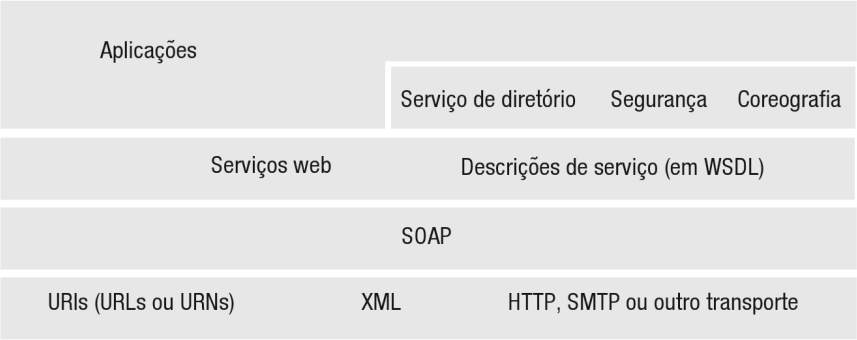
\includegraphics[scale=0.7]{./imagens/1_q_teorico/qt2.png}}
	\caption[Infraestrutura e componentes dos serviços
		\textit{web}. ]{Infraestrutura e componentes dos serviços
		\textit{web}. \textbf{Fonte:}\citeonline{coulouris2013}}
	\label{fig:ws}
\end{figure}
	
	\par Os \textit{web services} geralmente fazem uso do protocolo SOAP, para
estruturar e encapsular as mensagens trocadas. De acordo com
\citeonline[p.381]{coulouris2013}, "o protocolo SOAP é projetado para permitir
tanto interação cliente-servidor de forma assíncrona pela Internet". Segundo
\citeonline[p.27]{sampaio2006}, "o SOAP foi criado inicialmente, para
possibilitar a invocação remota de métodos através da internet".

	\par As mensagens SOAP possuem um elemento envelope, que de acordo com
\citeonline[p.19]{saudate2013}, "é puramente um \textit{container} para os
elementos \textit{Header} e \textit{Body}". O elemento \textit{header}
transporta metadados relativos à requisição tais como autenticação, endereço de
retorno da mensagem, etc. Já o elemento \textit{body} carrega o corpo da
requisição, que nada mais é do que o nome da operação e paramêtros referentes à
mesma. É válido lembrar que todas requisições são trocadas usando SOAP, e usam
o XML como formato oficial. 
%Na Figura \ref{fig:qt3} está representado o esquema do Envelope SOAP.
	
%\begin{figure}[h!]
%	\centerline{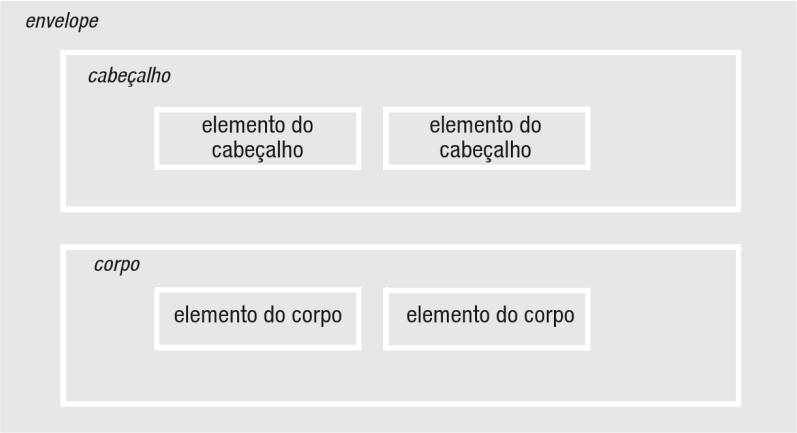
\includegraphics[scale=0.6]{./imagens/1_q_teorico/qt3.png}}
%	\caption[Esquema de envelope SOAP. ]{Esquema de envelope SOAP. 
%	 \textbf{Fonte:}\citeonline{coulouris2013}}
%	\label{fig:qt3}
%\end{figure}

	\par Os \textit{web services}, além de fornecerem uma padronização de
comunicação entre as várias tecnologias existentes, proveem transparência na
troca de informações. Isso contribui para que as novas aplicações consigam se
comunicar com aplicações mais antigas ou aplicações construídas sobre outras
plataformas.

	\par Além das tecnologias \textit{web services} tradicionais, existem os
\textit{web services} REST que também disponibilizam serviços, porém não
necessitam de encapsulamento de suas mensagens assim como os \textit{web
services} SOAP. Este fato influencia diretamente na \textit{performance} da
aplicação, haja vista que não sendo necessário o encapsulamento da informação
requisitada ao \textit{web service}, somente é necessário o processamento e
tráfego da informação que realmente importa. As caracteristícas do padrão REST
serão abordadas na próxima seção.

			%rest
			\subsection{REST}
				\subsection{REST}
	
	\par Segundo \citeonline{saudate2012}, REST\footnote{REST
-\textit{Representational State Transfer} ou Transferência de Estado
Representativo.}, desenvolvido por Roy Fielding na defesa de sua tese de
doutorado. Segundo o próprio \citeonline{fielding2000} REST é um estilo que
deriva dos vários estilos arquitetônicos baseados em rede e  que combinado com
algumas restrições, fornecem uma interface simples e uniforme para fornecimento
de serviços\footnote{Tradução e resumo de informações de responsabilidade dos
autores da pesquisa.}.
			
	\par \citeonline{rubbo2015} afirma que os dados e funcionalidades de um sistema
são considerados recursos e podem ser acessados através das URI's
\textit{(Universal Resource Identifier)}, facilitando dessa forma a comunicação
do servidor com o cliente. Um serviço contruído na arquitetura REST basea-se
fortemente em recursos. \citeonline{saudate2012}, explica ainda que os métodos
do HTTP podem fazer modificações nos recursos, da seguinte forma:
	
	\begin{itemize}
		\item GET: para recuperar algum dado. 
		\item POST: para criar algum dado.
		\item PUT: para alterar algum dado. 
		\item DELETE: para excluir algum dado. 
	\end{itemize}

	\par Como o próprio \citeonline{fielding2000} também foi um dos criadores de
um dos protocolos mais usados na web, o HTTP, pode-se dizer que o REST foi
concebido para rodar sobre esse protocolo com a adição de mais algumas
características que segundo \citeonline{saudate2013}, foram responsáveis pelo
sucesso da web:
		
	\begin{itemize}
		\item URLs bem definidas para recursos;
		\item Utilização dos métodos HTTP de acordo com seus propósitos;
		\item Utilização de \textit{media types} efetiva;
		\item Utilização de \textit{headers} HTTP de maneira efetiva;
		\item Utilização de códigos de \textit{status} HTTP;
	\end{itemize}
			 
	\par Segundo \citeonline{godinho2009}, não há um padrão de formato para as
 trocas de informações, mas as que mais são utilizadas é o XML\footnote{XML
 - \textit{Extensible Markup Language}.} e o JSON\footnote{JSON - 
 \textit{JavaScript Object Notation}.}. O REST é o mais indicado para aplicações
 em dispositivos móveis, devido a agilidade que proporciona na comunicação
 entre cliente e servidor.

	%tomcat
	\section{Apache Tomcat}
		\section{\textit{Apache Tomcat}}

	\par De acordo com \citeonline{tomcat2015}, \textit{Apache Tomcat} é uma
implementação de código aberto das especificações \textit{Java Servlet} e
\textit{JavaServer Pages}. O \textit{Apache Tomcat} é um \textit{Servlet
Container}, que disponibiliza serviços através de requisições e respostas.
\citeonline{caelum2} afirma que ele utilizado para aplicações que necessitam
apenas da parte \textit{Web} do Java EE\footnote{EE - Sigla para enterprise
edition}.

	\par Segundo \citeonline{tomcat2015}, o projeto desse \textit{software}
começou com a \textit{Sun Microsystems}, que em 1999 doou a base do código para
\textit{Apache Software Foundation}, e então seria lançada a versão 3.0.

	\par Conforme \citeonline{devMedia2015}, para o desenvolvimento com
	\textit{Tomcat} é necessária a utilização das seguintes técnologias:
	
	\begin{itemize}
	  
	  \item JAVA: é utilizado em toda parte lógica da aplicação.
	  
	  \item HTML: é utilizado na parte de interação com o usuário.
	  
	  \item XML: é utilizado para as configurações do \textit{software}. 
	
	\end{itemize}
 
 
 
	\par Desta forma, o cliente envia uma requisição através do seu navegador, o
servidor por sua vez a recebe, executa o \textit{servlet} e devolve a resposta
ao usuário.
	
	%postgres
	\section{PostgreSQL}
		\section{PostgreSQL}

	\par Para \citeonline{milani2008}, todas as aplicações que armazenam
informações para o seu uso posterior devem estar integradas a um banco de
dados, seja armazenando em arquivos de textos ou em tabelas. Por isso, o
\textit{PostgreSql} tem por finalidade armazenar e administrar os dados em uma
solução de informática.
	
	\par \citeonline[s.p]{postgresWiki2015} define que “o \textit{PostgreSql} é
um SGBD (Sistema Gerenciador de Banco de Dados) objeto-relacional de código
aberto, com mais de 15 anos de desenvolvimento. É extremamente robusto e
confiável, além de ser extremamente flexível e rico em recursos.” 

	\par Conforme afirma \citeonline{milani2008}, o PostgreSql é um
SGDB\footnote{SGDB - Sistema Gerenciador de Banco de Dados } de código aberto
originado na Universidade de \textit{Berkeley}, na Califórnia (EUA) no ano de
1986, pelo projeto \textit{Postgres} desenvolvido por uma equipe sob liderança
do professor Michael Stonebraker. Ele possui os principais recursos dos bancos
de dados pagos e está disponível para os sistemas operacionais
\textit{Windows}, \textit{Linux} e \textit{Mac}. Atualmente existem bibliotecas
e \textit{drivers} para um grande número de linguagens de programação, entre as
quais podemos citar: C/C++, PHP, \textit{Java}, ASP, \textit{Python} etc.

	\par De acordo com \citeonline{postgres2015}, existem sistemas com o
\textit{PostgreSql} que gerenciam até quatro \textit{terabytes} de dados. Seu
banco não possui um tamanho máximo e nem um número máximo de linhas por tabela.
Contudo, uma tabela pode chegar a ter um tamanho de trinta e dois
\textit{terabytes} e cada campo a um \textit{gigabyte} de informação.

	\par Segundo \citeonline{milani2008}, são características do
\textit{PostgreSql}:

	\begin{itemize}
	  
	  \item Suporte a ACID (Atomicidade, Consistência, Isolamento e Durabilidade). 
	  
	  \item Replicação de dados entre servidores.
	  
	  \item Cluster.
	  
	  \item Multithreads.
	  
	  \item Segurança SSL\footnote{SSL -\textit{Secure Socket Layer}} e
	  criptografia.
	    
	\end{itemize}

	\par É através do \textit{PostgreSql} que o \textit{webservice} armazenará e
posteriormente retornará os dados dos discentes para o aplicativo
\textit{Andorid}.
	
	%uml
	\section{UML}
		\section{UML}
		
	\par De acordo com \citeonline{booch2006uml} "A UML (\textit{Unified Modeling
Language}) é uma linguagem-padrão para a elaboração da estrutura de projetos
de \textit{software}". Na decada de 80 seguindo o surgimento e a evolução das
linguagens de programação orientadas a objetos, foram surgindo linguagens de
modelagens orientadas a objetos, como um modo alternativo de análise e projeto
de \textit{software} usadas na época. De acordo com
\citeonline[p.19]{guedes2011}:
	\begin{citacao}
		A UML surgiu da união de três métodos de modelagem: o método de Booch, o
		método OMT (\textit{Object Modeling Technique}) de Jacobson, e o método OOSE
		(\textit{Object-Oriented Software Engineering}) de Rumbaugh. Estes eram, até
		meados da década de 1990, os métodos de modelagem orientada a objetos mais
		populares entre os profissionais da área de desenvolvimento de
		\textit{software}. A união desses métodos contou com o amplo apoio da
		\textit{Rational Software}, que a incentivou e financiou.
	\end{citacao}

	\par Segundo \citeonline[p.13]{booch2006uml} "A UML é independente de processo,
apesar de ser perfeitamente utilizada em processo orientado a casos de usos,
centrado na arquitetura, interativo e incremental". A linguagem de modelagem
UML, além de fornecer um vocabulário próprio, também provê uma série de
diagramas que tem inúmeras finalidades diferentes. Tais finalidades e suas
subdivisões estão representados na Figura \ref{fig:qt4}.
		
	\begin{figure}[h!]
		\centerline{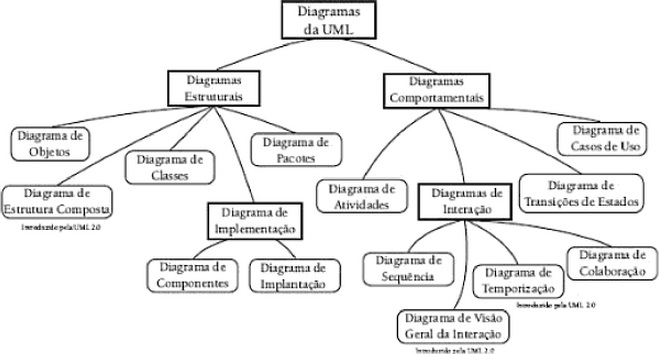
\includegraphics[scale=1]{./imagens/1_q_teorico/qt4.png}}
		\caption[Principais Diagramas definidos pela UML.]{Diagramas definidos pela
		UML. \textbf{Fonte:}\citeonline{2015principios}}
		\label{fig:qt4}
	\end{figure}
	\pagebreak
	
	\par A linguagem de modelagem UML não é processo rígido e permite uma
adequação de acordo com a situação do projeto em que é aplicada. Por permitir
essa flexibilidade e prover suporte adequado para determinados casos de um
projeto, será utilizada a linguagem de modelagem UML  para o desenvolvimento
desta pesquisa.
	
	%gcm
	\section{Google Cloud 	Messaging}
		%\section{\textbf{Google Cloud 	Messaging}}

	\par Para que os alunos sejam notificados quando houver alguma mudança no
portal do aluno, será utilizada uma API oferecida pela Google denominada
\textit{Google Cloud Messaging} ou simplesmente GCM, um recurso que tem por
objetivo notificar as aplicações \textit{Android}. Segundo \citeonline{leal2014}, ele
permite que aplicações servidoras possam enviar pequenas mensagens de até 4
KB\footnote{\textit{KB - Kilobytes}} para os aplicativos móveis, sem que este
necessite estar em execução. Ainda de acordo com \citeonline{leal2014} para o
bom funcionamento do recurso apresentado, são necessários os seguintes
componentes:

\begin{itemize}
	
	\item \textit{Sender ID\footnote{Identity}}: é o identificador do projeto.
	Será utilizado pelo servidores da Google para identificar a aplicação
	que envia a mensagem.
	
	\item \textit{Application ID}: é o identificador da aplicação \textit{Android}. O
	identificador é o nome do pacote do projeto que consta no
	\texttt{AndroidManifest.xml}.
	
	\item \textit{Registration ID}: é o identificador gerado pelo servidor GCM
	quando aplicação \textit{Android} se conecta a ele. Este deve ser enviado
	também à aplicação servidora.
	
	\item \textit{Sender Auth Token}: é uma chave que é incluída no cabeçalho
	quando a mensagem é enviada da aplicação servidora para o GCM. Essa chave serve
	para que a API da Google possa enviar as mensagens para o dispositivo
	correto.

\end{itemize}

	\par De acordo com os componentes acima citados, quando uma aplicação servidora
enviar uma mensagem para o aplicativo \textit{Android}, na verdade está
enviando para o servidor GCM que será encarregado de enviar a mensagem para a aplicação
\textit{mobile}.

	
	%jersey
	\section{Jersey}
		%\section{\textit{Jersey}}

	\par Atualmente um padrão para desenvolvimento de serviços \textit{web} vem
sendo bastante adotado, trata-se do padrão arquitetural REST. De acordo com
\citeonline{saudate2012}, a linguagem \textit{Java} possui uma especificação
própria para desenvolvimento de serviços REST desde de setembro de 2008, que é
a JSR311, ou como é popularmente chamado JAX-RS. Esta especificação provê um
conjunto de API's simples, para facilitar o desenvolvimento de serviços
\textit{web}. De acordo com \citeonline{oracle22015} "JAX-RS é uma API da
linguagem de programação \textit{Java} projetada para tornar mais fácil
desenvolver aplicações que usam a arquitetura REST"\footnote{Tradução e resumo
de informações de responsabilidade dos autores da pesquisa.}. Através desta
especificação torna-se mais facíl e ágil a contrução de serviços \textit{web}
baseados em REST.

	\par Como JAX-RS é apenas uma especificação, ela necessita então de uma
implementação. Uma das implementações desta especificação é o
\textit{framework Jersey}. Segundo \citeonline{oracle2015} "\textit{Jersey}, a
implementação de referência de JAX-RS, implementa suporte para as anotações
definidas no JSR 311, tornando mais fácil para os desenvolvedores a construir
serviços \textit{Web RESTful} usando a linguagem de programação
\textit{Java}"\footnote{Tradução e resumo de informações de responsabilidade
dos autores da pesquisa.}. Além das anotações que facilitam seu uso,
\textit{Jersey} pode prover serviços com uma infinidade de tipos de
mídias, tais como XML e JSON entre outros.

	\par O \textit{framework Jersey} tem amplo suporte para os varios métodos HTTP.
Fazendo uso dele pode-se facilmente implementar recursos REST. Além disso o
\textit{Jersey}  pode rodar tanto em servidores que implementem a especificação
\textit{Servlet} ou não. Este \textit{framework} será usado para contruir a
parte responsável por prover os serviços para o aplicativo \textit{Android}.
	
	%hibernate
	\section{Hibernate}
		%\section{Hibernate}

	\par Com a evolução e popularização da linguagem Java, e com o seu
uso cada vez maior em ambientes corporativos, percebeu-se que se perdia muito
tempo com a confecção de \textit{queries} SQL usadas nas consultas em bancos de
dados relacionais e com a construção do código JDBC\footnote{JDBC -
\textit{Java Database Connectivity}}, que era responsável por trabalhar com
estas consultas. Além disso era notório que, mesmo a linguagem SQL sendo
padronizada, ela apresentava diferenças significativas entre os diversos bancos
de dados existentes. Isso fazia com que a implementação de um software ficasse
amarrada em um banco de dados específico e era extremamente custosa uma mudança
poterior. Além disso havia o problema de lidar diretamente com dois paradigmas
um pouco diferentes: o orientado a objeto e o relacional. Com o intuito de
resolver estes problemas, é que surgiram os \textit{frameworks}
ORM\footnote{ORM - \textit{Object-relational Mapping}} tais como Hibernate,
EclipseLink, Apache OpenJPA entre outros.

	\par Conforme surgiam novas alternativas e implementações para sanar esses
problemas, surgia um novo problema: a falta de padronização entre os
\textit{frameworks} de ORM. Para resolver esse problema foi criada o
JPA\footnote{JPA - \textit{Java Persistence API}} que, de acordo com
\citeonline[p.12]{keith2009pro}, "nasceu do reconhecimento das demandas dos
profissionais e as existentes soluções proprietárias que eles estavam usando
para resolver os seus problemas"\footnote{Tradução de responsabilidade dos
autores da pesquisa.}. 
	
	\par A especificação JPA foi concebida sendo a terceira parte da
especificação EJB\footnote{EJB - \textit{Enterprise Java Bean}}, e deveria
atender ao propósitos de persistêcia de dados desta especificação.
De acordo com \citeonline[p.12]{keith2009pro}, JPA é um \textit{framework} leve
baseado em POJO's\footnote{POJO - \textit{Plain Old Java Object }}, para
persistência de dados em Java e que, embora o mapeamento objeto
relacional seja seu principal componente, ele ainda oferece soluções de
arquitetura para aplicações corporativas escaláveis\footnote{Tradução e resumo
de informações de responsabilidade dos autores da pesquisa.}.

	\par O \textit{framework} Hibernate é uma das implementações da especificação
JPA. De acordo com \citeonline{sourceforgeHibernate2015}, o Hibernate é
uma ferramenta de mapeamento relacional, muito popular entre aplicações
Java e implementa a \textit{Java Persistence API}. Foi criado por uma
comunidade de desenvolvedores, do mundo todo, que eram liderados por Gavin King.
De acordo com \citeonline{hibernate2015} "o Hibernate cuida do mapeamento
de classes Java para tabelas de banco de dados, e de tipos de dados
Java para tipos de dados SQL".

	\par O Hibernate está bastante difundido na comunidade de desenvolvedores Java
ao redor do mundo, pelo fato de ser simples de usar e por evitar esforços
desnecessários na parte de infraestrutura das aplicações onde é usado, mantendo
assim o foco na lógica de negócio. As pricipais vantagens do uso do Hibernate,
segundo \citeonline{sourceforgeHibernate2015}, são:

	\begin{itemize}
	  
		\item Provedor JPA: além de sua API nativa , o Hibernate também é uma
		implentação da especificação JPA, podendo assim ser facilmente usado em
		qualquer ambiente JPA.
		  		
		\item Persistência idiomática: permite que sejam construídas classes
		persistentes, e que suportem herança e polimorfismo entre outras estratégias,
		sem a necessidade da contrução de estruturas especiais para tal fim.
			  	
		\item \textit{Performance} e suporte: permite que sejam usadas várias
		estratégias de inicialização. Além disso não necessita de tabelas especiais
		no banco de dados. Mostra-se vantajoso também por gerar a maior parte do SQL
		necessário e evitar esforço desnecessário por parte do desenvolvedor, além de
		ser mais rápido que o JDBC puro.
		  
		\item Escalável: o Hibernate foi projetado para trabalhar em
		\textit{clusters} de servidores de aplicações e oferecer uma estrutura muito
		escalável, que se comporta bem tanto com número pequeno de usuários até
		números mais elevados.
	
		\item Confiável: sua confiabilidade e estabilidade são comprovadas pelo seu
		grande uso e aceitação atualmente.
				
		\item Extensível: Hibernate é altamente configurável e
		extensível\footnote{Tradução e resumo de informações de responsabilidade dos
		autores da pesquisa.}.
	
	\end{itemize}
	
	\par O Hibernate será usado nesta pesquisa com o intuito de fazer a
gerência dos dados coletados e que serão providos para o aplicativo
Android através do \textit{web service}, em conjunto com o banco de
dados.
		
		%Maven
	\section{Maven}
		%\section{Maven}

%conteudos retirados como exigencia da banca avaliadora	
%\section{Engenharia de \textit{Software}}

	\par De acordo com \citeonline{carvalho2001}, a engenharia de \textit{software}
surgiu na década de 80, com intuito de melhorar o desenvolvimento de
\textit{software}, produzindo sistemas de alta qualidade com a redução do custo
e do tempo.

	\par Segundo \citeonline[p.39]{pressman2011}, engenharia de \textit{software} é
“o estabelecimento e o emprego de sólidos princípios da engenharia de modo a
obter \textit{software} de maneira econômica, que seja confiável e funcione de
forma eficiente em máquinas reais”.

	\par Como afirmam \citeonline{carvalho2001}, a engenharia possui modelos de
processos que possibilitam ao gerente controlar o desenvolvimento e aos
programadores uma base para produzir. Alguns desses paradigmas são:

	\begin{itemize}
	  
	  \item Ciclo de vida clássico: utiliza o método sequencial, em que o final
	  de uma fase é o início da outra.
	  
	  \item O paradigma evolutivo: baseia-se no desenvolvimento e implementação
	  de um produto inicial. Esse produto passa por críticas dos usuários e vai
	  recebendo melhorias e versões até chegar ao produto desejado.
	  
	  \item O paradigma espiral: engloba as melhores características do ciclo de
	  vida clássica e o paradigma evolutivo. Ele consiste em vá - rios ciclos e
	  cada ciclo representa uma fase do pesquisa.
	
	\end{itemize}



	\par De toda a engenharia de \textit{software}, o que mais será utilizado nesse
projeto é a linguagem UML, que através dos seus diagramas norteará os caminhos
a serem seguidos.
%\subsection{Processos de \textit{Software}}
	
	
	\par Segundo \citeonline[p.52]{pressman2011}, um processo de \textit{software} é
“uma metodologia para as atividades, ações e tarefas necessárias para
desenvolver um \textit{software} de alta qualidade”.

	\par Para \citeonline{sommerville2003}, não existe um processo ideal, pois isso
dependerá de cada projeto, possibilitando cada qual implementar algum modelo já
existente. Contudo \citeonline{pressman2011} afirma que uma metodologia
genérica possui cinco passos:
	\begin{itemize}
	  
	  \item Comunicação: antes de iniciar os trabalhos técnicos deve-se entender
	  os objetivos do sistema e levantar requisitos para o bom funcionamento do
	  \textit{software}.
	  
	  \item Planejamento: cria um plano de projeto, que conterá as tarefas a
	  serem seguidas, riscos prováveis e recursos necessários.
	  
	  \item Modelagem: esboça o sistema para que se tenha uma ideia de como ele
	  deverá ficar e como encontrar a melhor solução para desenvolvê-lo.
	  
	  \item Construção: é a etapa de desenvolvimento e testes.
	  
	  \item Emprego: o \textit{software} pronto em sua totalidade ou parcialmente
	  é implantado no cliente e este retorna o seu \textit{feedback}.
	 
	 \end{itemize}
	 
	 \par Dessa forma, normalmente qualquer um dos modelos (ciclo de vida clássico,
evolutivo ou espiral) utilizaram os princípios das metodologias acima citadas.
	



				





